\documentclass[11pt]{article}
\usepackage[margin=0.95in]{geometry}
\usepackage{amsmath,amssymb,amsthm,mathtools}
\usepackage{graphicx,booktabs,xcolor,microtype,enumitem,caption,subcaption}
\usepackage[numbers,sort&compress]{natbib}
\usepackage{placeins}
\usepackage[colorlinks=true,linkcolor=black,citecolor=blue!50!black,urlcolor=blue!50!black]{hyperref}
\graphicspath{{../figures/}}
\captionsetup{font=small,labelfont=bf}
\setlist{itemsep=1pt,topsep=3pt}
\renewcommand{\topfraction}{0.9}\renewcommand{\bottomfraction}{0.6}\renewcommand{\textfraction}{0.08}\renewcommand{\floatpagefraction}{0.85}
\newtheorem{theorem}{Theorem}
\newtheorem{lemma}[theorem]{Lemma}
\newtheorem{proposition}[theorem]{Proposition}
\theoremstyle{definition}
\newtheorem{observation}[theorem]{Observation}

\title{\textbf{The Wrong Gradient}\\[3pt]
\large Potential games, marginal costs, and where the game stops describing the boats}
\author{Liam Kenji Bray\thanks{RoboBoat team, computer-science lead.}}
\date{November 2026}

\begin{document}
\maketitle

\begin{abstract}
\noindent When each autonomous boat in a fleet does what is best for itself, the fleet as a whole descends the wrong landscape. In congestion games this is exact. Selfish moves lower Rosenthal's potential $\Phi$, an area under a staircase, while the fleet pays the enclosing rectangle $C$. The gap is the delay each newcomer imposes on the others. Charging each boat the discrete derivative of an edge's total cost closes it: the potential then telescopes to $C$, a discrete fundamental theorem of calculus. Whether a game has a potential at all is a loop condition, a discrete analogue of a curl-free vector field. We test how far these exact statements survive in a simulated fleet of twin-thruster boats with currents, queues, camera and lidar perception and a lossy radio, on courses modelled on the RoboBoat autonomy challenge. We built Braess's paradox into the course and calibrated the game from the boats themselves. With single-file channels the predicted paradox reversed: an upstream queue spaces boats out and pre-pays the downstream one. The measured route game violates the exact-potential condition, with four-cycle circulations six times their noise, and exhibits a strict improvement cycle, ruling out even an improvement-preserving potential for that finite model. With congestion that slows boats together, the paradox appeared. In task allocation, better travel-time models did not change decisions (a preregistered null on 400 worlds). Rules that discount stale teammate claims undercharge the difference-reward toll and cause duplicated trips: on 200 courses, the more readily a rule doubted a claim, the more points the fleet lost. Coordination strategy mattered with four boats but not with two, the fleet size the 2026 rules allow, and a central planner's advantage came mostly from privileged information.
\end{abstract}

% =====================================================================================
\section{Introduction}
\label{sec:intro}
Four autonomous boats leave a dock for an inspection area. There are two routes: one goes through a narrow canal and then open water, the other through open water and then a second canal. Each canal takes $2k$ minutes when $k$ boats use it; each open-water leg takes 10 minutes regardless. Split two and two, every boat takes 14 minutes and the fleet spends 56 boat-minutes, the best it can do. Now open a one-minute shortcut joining the end of the first canal to the start of the second. One boat saves three minutes by taking canal, shortcut, canal, and the fleet's total rises to 57. The other three boats make the same rational switch, one at a time, and the fleet settles at 68 boat-minutes, in a state that no boat can improve by moving alone. Adding a road made everyone slower. This is Braess's paradox~\cite{braess1968,braess2005}.

The paradox has an exact explanation, and it gives this paper its title. When each boat improves its own travel time, the fleet does descend a landscape, but it is the wrong one. Every selfish improvement lowers a quantity called Rosenthal's potential $\Phi$, while the fleet pays a different quantity, the total cost $C$. The boats follow the gradient of $\Phi$, in the discrete sense of always moving downhill on it, and the gap between $\Phi$ and $C$ is exactly the delay each boat imposes on the others. Charging each boat the \emph{discrete derivative} of an edge's total cost (its own delay plus a toll for the delay it causes) closes the gap, and the proof that it does is the fundamental theorem of calculus in discrete form.

The question we pursue is what happens to these exact statements when the players are physical robots. Our boats obey differential equations with turning limits and water currents. They queue at narrow gates, find tasks only through simulated cameras and lidar, and coordinate over a radio that loses messages in bursts. We built a simulator of such a fleet on a course modelled on the RoboBoat autonomy challenge~\cite{robonation2025}. From 2026 the competition admits up to two vehicles per team and invites inter-vehicle communication~\cite{robonation2026}, so coordinating a small fleet is a real engineering question. We ask three questions:
\begin{enumerate}
\item When does the abstract game describe the physical fleet? We built Braess's harbour into the course and calibrated the game from the boats themselves. The prediction failed because travel times depend on traffic \emph{elsewhere} (\S\ref{sec:q1}).
\item Does modelling the physics or the information better help a fleet that decides locally? Better travel-time estimates did not. Plausible ways of handling stale messages made things worse; we traced why, and the best rule was not to discount teammates' claims at all (\S\ref{sec:q2}).
\item When does the structure of coordination matter, and what should a two-boat entry do? It depends on fleet size, and on whether a central planner's advantage comes from better optimization or from better information (\S\ref{sec:q3}).
\end{enumerate}

The mathematical tools come from a well-developed theory. Rosenthal showed that congestion games always have a potential~\cite{rosenthal1973}; Monderer and Shapley characterized exactly which games do~\cite{monderer1996}; the price of anarchy measures how much selfishness costs~\cite{roughgarden2002}; and marginal-cost tolls and difference rewards are the standard ways to align individual and collective incentives~\cite{wolpert2001,wolpert2002,marden2009}. Multi-robot task allocation borrows these ideas through auctions and assignment~\cite{gerkey2004,choi2009}. The theory assumes clean costs and correct information. This study asks what happens when it meets boats that obey differential equations and talk over a lossy radio. It does so with a simulator that keeps a strict boundary between what is true and what each boat knows, with paired experiments on hundreds of generated courses, and with a direct test of whether the boats' measured costs still form a potential game.

% =====================================================================================
\section{The mathematics of selfish fleets}
\label{sec:math}

\subsection{Two functions on the same profiles}
Boats $i=1,\dots,n$ each choose a path $a_i$, a set of edges, through a directed graph. In the harbour (Fig.~\ref{fig:braess}a) boats travel from the dock $S$ to the inspection area $T$; $A$ and $B$ are the two junctions where a canal meets an open-water leg. A boat can take \mbox{$S\!\to\!A\!\to\!T$} or \mbox{$S\!\to\!B\!\to\!T$}, or, once the shortcut is open, the zigzag \mbox{$S\!\to\!A\!\to\!B\!\to\!T$}. A \emph{profile} $a=(a_1,\dots,a_n)$ lists every boat's choice. The load $n_e(a)$ is the number of boats using edge $e$, and $c_e(k)$ is the time on edge $e$ when $k$ boats use it. Boat $i$ pays the sum of its edges' times, and the fleet pays the sum over boats, which regroups by edge:
\begin{equation}
c_i(a)=\sum_{e\in a_i}c_e\big(n_e(a)\big),\qquad
C(a)=\sum_i c_i(a)=\sum_e n_e(a)\,c_e\big(n_e(a)\big). \label{eq:C}
\end{equation}
A boat's \emph{best response} is the path that minimizes its own cost with everyone else's paths held fixed. A profile is a \emph{Nash equilibrium} if every boat is already playing a best response, so that no boat can lower its own cost by changing only its own path, and the \emph{price of anarchy} (PoA) is the worst equilibrium's cost divided by the optimum. Rosenthal observed that one function tracks every boat's private incentive at once:
\begin{equation}
\Phi(a)=\sum_e\sum_{k=1}^{n_e(a)}c_e(k). \label{eq:Phi}
\end{equation}

\begin{theorem}[Rosenthal~\cite{rosenthal1973}]\label{thm:rosenthal}
$\Phi$ is an exact potential: whenever a single boat $i$ changes its path, the change in $\Phi$ equals the change in $i$'s own cost, $\Delta\Phi=\Delta c_i$.
\end{theorem}
\begin{proof}
Let $i$ move from $P$ to $Q$, with loads $\ell_e$ before the move. Edges on both paths, or on neither, keep their load and change nothing. An edge $i$ leaves drops from $\ell_e$ to $\ell_e-1$ boats, so its inner sum in \eqref{eq:Phi} loses its last term, $c_e(\ell_e)$, which is what $i$ was paying there. An edge $i$ joins gains the term $c_e(\ell_e+1)$, which is what $i$ will pay there. Hence $\Delta\Phi=\sum_{Q\setminus P}c_e(\ell_e+1)-\sum_{P\setminus Q}c_e(\ell_e)=\Delta c_i$.
\end{proof}
Every selfish improvement lowers $\Phi$, and $\Phi$ takes finitely many values, so boats that improve one at a time must stop, and they stop at a Nash equilibrium. In the harbour, the first switch lowers boat 1's time from 14 to 11 and $\Phi$ from 52 to 49; four switches take $\Phi$ from 52 to 44 while $C$ climbs from 56 to 68 (Fig.~\ref{fig:braess}c).

There is a simple picture of the difference. Draw $c_e$ as a staircase of unit-width steps (Fig.~\ref{fig:braess}b). The edge's contribution to $\Phi$ is the \emph{area under the staircase} up to $n_e$, while its contribution to $C$ is the \emph{rectangle} $n_e\times c_e(n_e)$: every boat on the edge pays the current, highest step. Selfish boats minimize area, the fleet pays rectangles, and the difference is the region inside the rectangle but above the staircase: the extra delay that every earlier boat suffers because later boats joined. For affine costs $c_e(k)=\alpha_e k+\beta_e$ the area has a closed form,
\[
\sum_{k=1}^{n}(\alpha k+\beta)=\alpha\frac{n(n+1)}{2}+\beta n=\frac12\Big[n(\alpha n+\beta)+n(\alpha+\beta)\Big]=\frac12\Big[n\,c(n)+n\,c(1)\Big],
\]
and summing over edges gives
\begin{equation}
\Phi=\tfrac12\Big[C+\textstyle\sum_i c_i^{\rm alone}\Big],\qquad c_i^{\rm alone}=\sum_{e\in a_i}c_e(1). \label{eq:half}
\end{equation}
Selfish boats minimize the \emph{average} of the true fleet cost and an ``empty-harbour'' cost. The zigzag costs only $2+1+2=5$ minutes on an empty harbour, against 12 for the other routes, so $\Phi$ rewards it even though $C$ punishes it.

\begin{figure}[t]
\centering
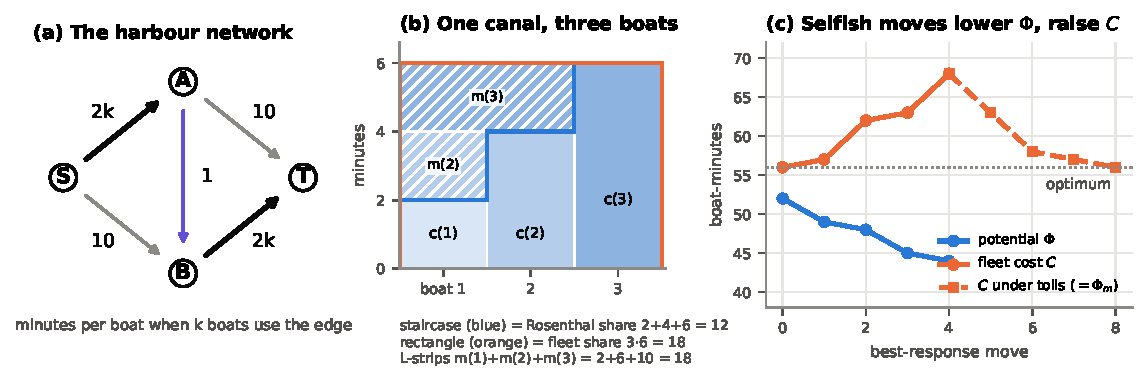
\includegraphics[width=\linewidth]{fig1_braess.pdf}
\caption{\textbf{(a)} The harbour network: boats go from the dock $S$ to the inspection area $T$ through junctions $A$ and $B$; edge labels are minutes per boat with $k$ boats on the edge, and the violet edge is the shortcut. \textbf{(b)} One canal ($c(k)=2k$) carrying three boats. The staircase (blue) is the canal's share of Rosenthal's potential; the rectangle (orange) is its share of the fleet cost. The rectangle splits into L-shaped strips $m(k)$: a boat's own column $c(k)$ plus the hatched delay it adds to the boats already there. Their sum telescopes to the rectangle. \textbf{(c)} Boats switching one at a time to their best response after the shortcut opens: $\Phi$ falls $52\!\to\!44$ while $C$ rises $56\!\to\!68$. Dashed: the true $C$ when boats respond to marginal-cost tolls, which returns to the optimum.}
\label{fig:braess}
\end{figure}

\subsection{Where the paradox comes from}
\begin{lemma}[Externality decomposition]\label{lem:ext}
For the same move $P\to Q$,
\begin{equation}
\Delta C = \Delta c_i + \underbrace{\sum_{e\in Q\setminus P}\ell_e\big[c_e(\ell_e{+}1)-c_e(\ell_e)\big]}_{\text{delay imposed on the boats already there}} - \underbrace{\sum_{e\in P\setminus Q}(\ell_e{-}1)\big[c_e(\ell_e)-c_e(\ell_e{-}1)\big]}_{\text{relief given to the boats left behind}}.
\label{eq:ext}
\end{equation}
\end{lemma}
\begin{proof}
On a joined edge the rectangle grows from $\ell c(\ell)$ to $(\ell+1)c(\ell+1)=c(\ell+1)+\ell\,c(\ell+1)$, an increase of $c(\ell+1)+\ell[c(\ell+1)-c(\ell)]$: the mover's new payment plus a raise for each of the $\ell$ boats already there. On a left edge it shrinks by $c(\ell)+(\ell-1)[c(\ell)-c(\ell-1)]$. The mover's own payments add up to $\Delta c_i$ as in Theorem~\ref{thm:rosenthal}; what remains is the two sums.
\end{proof}
A boat sees only $\Delta c_i$. The fleet also pays the middle term. In the harbour's first move the boat joins the canal \mbox{$B\!\to\!T$}, which already carries two boats, and the empty shortcut; the edge it leaves, the open-water leg \mbox{$A\!\to\!T$}, has a constant cost. So $\Delta C=-3+2\,[c(3)-c(2)]=-3+4=+1$. The boat gains three minutes; the fleet loses one.

\subsection{Correcting the gradient: marginal cost as a discrete derivative}
If each boat paid for the delay it imposes, its private incentive would be the fleet's. Set $c_e(0)=0$ and let $F_e(k)=k\,c_e(k)$ be an edge's total cost with $k$ boats. Charge each user the toll $\tau_e(k)=(k-1)[c_e(k)-c_e(k-1)]$, so it effectively pays
\begin{equation}
m_e(k)=c_e(k)+\tau_e(k)=k\,c_e(k)-(k-1)\,c_e(k-1)=F_e(k)-F_e(k-1). \label{eq:m}
\end{equation}
\begin{theorem}[Marginal-cost pricing~\cite{roughgarden2002}]\label{thm:toll}
With tolls $\tau_e$, the game's potential equals the fleet cost: $\Phi_m=C$.
\end{theorem}
\begin{proof}
The tolled game is a congestion game with edge costs $m_e$, so by Theorem~\ref{thm:rosenthal} (whose proof never uses monotonicity) its potential is
\[
\Phi_m=\sum_e\sum_{k=1}^{n_e}\big[F_e(k)-F_e(k-1)\big]=\sum_e\big[F_e(n_e)-F_e(0)\big]=\sum_e n_e\,c_e(n_e)=C.\qedhere
\]
\end{proof}
This is the discrete fundamental theorem of calculus. The toll-inclusive price $m_e$ is the forward difference of the total cost $F_e$, and summing a difference telescopes back to the function, just as $\int_0^n F'(k)\,dk=F(n)-F(0)$. The continuous version shows what the price means: $\tfrac{d}{dk}\big[k\,c(k)\big]=c(k)+k\,c'(k)$, the boat's own delay plus the small extra delay $c'(k)$ it adds to each of the $k$ others. In Fig.~\ref{fig:braess}b the L-shaped strips are the $m(k)$; stacking them rebuilds the rectangle ($2+6+10=18$), while the staircase alone gives only $2+4+6=12$. In Lemma~\ref{lem:ext}, the imposed term is exactly the tolls the mover starts paying and the relief term is the tolls it stops paying, so $\Delta C=\Delta(c_i+\tau_i)$: under tolls every selfish improvement lowers $C$. That guarantees a profile that no single boat can improve, though not in general the global optimum; in the harbour, the tolled boats do return to the optimum of 56.

By exhaustive enumeration, the harbour without the shortcut has every equilibrium at the optimum. With it, exactly one of the $3^4=81$ profiles is an equilibrium: every boat on the zigzag at 17 minutes, so the price of anarchy is $68/56=17/14$.

The fleets studied later (\S\ref{sec:bench}) mostly choose tasks, not roads: which buoy course to run, which vessel to serve. The same accounting applies. Let $W(a)$ be the team's expected points, write $a_{-i}$ for everyone's choices except boat $i$'s, and give boat $i$ the \emph{difference reward} $u_i(a)=W(a)-W(a_{-i},\varnothing)$, the team's points with $i$ minus its points if $i$ did nothing. The subtracted term does not depend on $i$'s choice, so $\Delta u_i=\Delta W$ for every move of $i$: the team's welfare is an exact potential, one the boats push \emph{up}~\cite{wolpert2001,marden2009}. The difference reward is the task-allocation version of the toll: it charges a boat for value its teammates would have produced anyway. For one task worth $V$, with boat $i$ succeeding with probability $s_i$ and some teammate heading there succeeding with probability $s_{-i}$, independence gives
\begin{equation}
u_i=V\big[1-(1-s_i)(1-s_{-i})\big]-V s_{-i}=V\,s_i\,(1-s_{-i}).\label{eq:dr}
\end{equation}
A task that a teammate will surely finish ($s_{-i}\approx1$) is worth nothing to me, however valuable it is to the team. The identity holds for the \emph{true} $s_{-i}$; a boat that estimates it from stale messages charges itself the wrong toll.

\subsection{Potential games as conservative fields}
\label{sec:curl}
When does a game have an exact potential at all? Monderer and Shapley~\cite{monderer1996} answered with a loop condition. Take a profile $a$ and two boats $i,j$ with alternative choices $x,y$. Writing $(x,a_{-i})$ for the profile in which $i$ has switched to $x$ and everyone else is unchanged, walk around the closed four-cycle
\[
a \;\xrightarrow{\;i\to x\;}\; (x,a_{-i}) \;\xrightarrow{\;j\to y\;}\; (x,y,a_{-ij}) \;\xrightarrow{\;i\to a_i\;}\; (a_i,y,a_{-ij}) \;\xrightarrow{\;j\to a_j\;}\; a,
\]
adding up each mover's change in its own cost. Call the total the \emph{circulation} $I$. A finite game has an exact potential if and only if $I=0$ around every such four-cycle. If $\Phi$ exists, each step's cost change equals the step in $\Phi$, and a closed loop returns $\Phi$ to where it started.

The analogy with Calculus III is close. A vector field $\mathbf F$ is the gradient of a function exactly when $\oint\mathbf F\cdot d\mathbf r=0$ around every closed loop, and on a simply connected domain the test reduces to the cross-partials $\partial F_x/\partial y=\partial F_y/\partial x$. Writing $\Delta_i f$ for the change in a quantity $f$ when boat $i$ switches $a_i\to x$, and $\Delta_j f$ for the change when $j$ switches $a_j\to y$, the circulation rearranges to
\[
I=\Delta_i\big(\Delta_j c_j\big)-\Delta_j\big(\Delta_i c_i\big),
\]
the difference of two \emph{mixed second differences}: how much $j$'s cost change from switching depends on $i$'s choice, minus how much $i$'s depends on $j$'s. (Expanding the four steps gives this directly.) Unlike for vector fields, no connectivity condition is needed. A loop in which only one boat moves sums to zero automatically, since it just adds and subtracts that boat's own costs; and every closed path of single-boat moves can be built from such loops and four-cycles. An exact potential exists exactly when these cross-effects are symmetric, a discrete Clairaut condition. Congestion games pass the test automatically. A game that fails it is matching pennies, in which one player wants to match the other's choice of heads or tails and the other wants to differ (each wins or loses 2): its four-cycles have circulation $\pm8$, and it has no potential. In the harbour there are $1{,}944$ four-cycles (a starting profile, a pair of boats, and an alternative route for each), and every one has circulation exactly zero.

The continuous picture is Stokes's theorem: around a small square of side $\varepsilon$, $\oint\mathbf F\cdot d\mathbf r=\varepsilon^2(\partial_xF_y-\partial_yF_x)+O(\varepsilon^3)$, and the four-cycle circulation is the discrete version of that curl. A cousin from control theory is the Lie bracket: flowing along $f$, $g$, $-f$, $-g$ leaves the \emph{state} displaced by about $\varepsilon^2[f,g]$. In a game the profile always returns and what fails to cancel is the accumulated cost, so the analogy is to curl rather than to the bracket itself, and we use the bracket only as intuition. Circulation can also be computed from data: given the cost each boat actually experiences in each profile, we can ask whether the physical fleet still has a potential (\S\ref{sec:q1}).

% =====================================================================================
\section{From games to boats}
\label{sec:physics}
The game above assumes three things that a physical fleet does not give for free. Edge costs are known numbers $c_e(k)$; each edge's cost depends only on its own load; and players move one at a time knowing the current profile. Each breaks, and each break can be measured.

First, costs come from differential equations. Each boat is a twin-thruster catamaran with position $(x,y)$, heading $\psi$, forward speed $v$ and turn (yaw) rate $r$:
\begin{equation}
\dot x=v\cos\psi+c_x,\ \ \dot y=v\sin\psi+c_y,\ \ \dot\psi=r,\ \ \dot v=\tfrac{v_{\rm cmd}-v}{\tau_v}-k_d v|v|,\ \ \dot r=\tfrac{r_{\rm cmd}-r}{\tau_r},
\label{eq:boat}
\end{equation}
with water current $(c_x,c_y)$, response time constants $\tau_v,\tau_r$, quadratic drag $k_d$, and commands $v_{\rm cmd}=v_{\max}(T_L{+}T_R)/2$, $r_{\rm cmd}=r_{\max}(T_R{-}T_L)/2$, where $T_L,T_R\in[-1,1]$ are the left and right thrust commands and $v_{\max},r_{\max}$ the top speed and turn rate. It is integrated with the fourth-order Runge--Kutta method at time step $\Delta t=0.05$\,s; the model follows the standard manoeuvring form~\cite{fossen2011} without claiming to be a validated hull. The thrust map is a linear change of variables with a useful geometry. Because $\tfrac12|a+b|+\tfrac12|a-b|=\max(|a|,|b|)$ (take $a=T_L$, $b=T_R$), it sends the square $\|T\|_\infty\le1$ \emph{onto} the diamond $|v_{\rm cmd}|/v_{\max}+|r_{\rm cmd}|/r_{\max}\le1$. Full speed and full turn rate are opposite corners, so every unit of turning is paid for in forward speed. A route's travel time therefore depends on its shape, not just its length, and a boat must \emph{estimate} each edge cost. We compare a \emph{graph} estimate (path length over a calibrated cruise speed) with a \emph{control-aware} estimate that adds turn, current and stopping penalties measured by running the boats' own controller.

Second, costs are coupled through queues. A single-file buoy channel lets boats through one at a time, so it behaves like a server with a fixed service interval $h$, the headway between consecutive boats. A channel's delay then depends not only on how many boats use it but on how their arrivals are spaced, and that spacing is set by whatever they passed through upstream. An edge's cost becomes a function of the whole route profile, so the game is no longer \emph{separable} (each edge's cost depending only on its own load, as in \eqref{eq:C}), and the circulation of \S\ref{sec:curl} need not vanish.

Third, players act on stale beliefs. Boats find tasks with a simulated camera and lidar (a laser range-finder), and learn about teammates through a radio that switches between a good and a bad state (a two-state Markov loss model, the Gilbert--Elliott channel~\cite{gilbert1960,elliott1963}), so losses come in bursts, with 0.5--3\,s of latency. Every boat re-decides every 2\,s, simultaneously, on messages of varying age. The convergence argument of Theorem~\ref{thm:rosenthal} needs one-at-a-time moves; simultaneous moves on stale information can collide.

% =====================================================================================
\section{A RoboBoat-inspired fleet benchmark}
\label{sec:bench}
\begin{figure}[t]
\centering
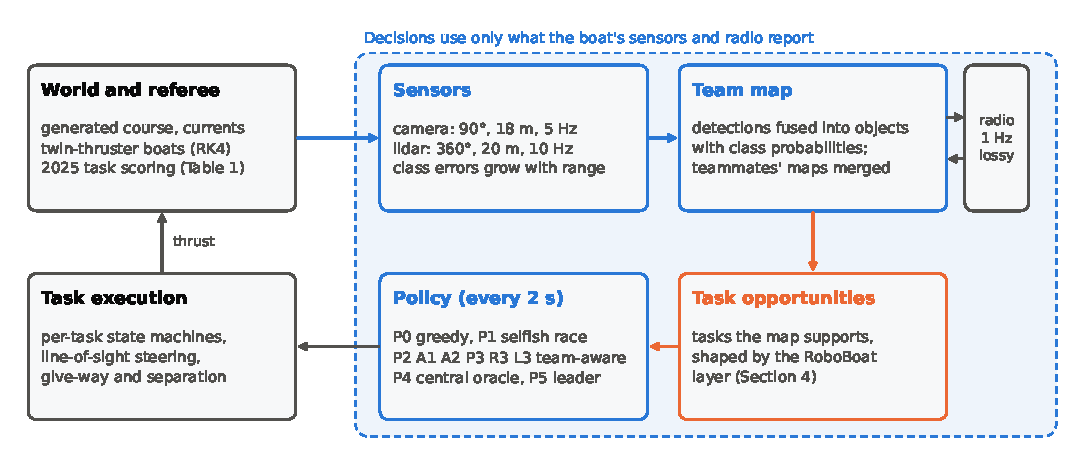
\includegraphics[width=\linewidth]{fig11_v2_architecture.pdf}
\caption{Simulator architecture. Everything inside the dashed boundary sees only sensor reports and received radio messages; a test verifies that perturbing hidden truth leaves decisions unchanged. All randomness (course, currents, sensor noise, packet loss) comes from named seeded streams, so every strategy faces identical inputs. Orange marks the coordination layer of \S\ref{sec:layer}.}
\label{fig:arch}
\end{figure}

The tasks and scoring follow sections 3.2 and 4.2 of the RoboBoat 2025 team handbook~\cite{robonation2025}. The 2026 edition replaces them with a new six-task scenario and allows two vehicles~\cite{robonation2026}; we keep the 2025 task set, which our simulator implements in full. The six tasks are: pass a navigation channel (T1); follow a path of gates while counting yellow buoys (T2); dock in the empty bay showing the banner of the day (T3); hold for a green light, then circle a blue buoy against the clock (T4); spray or deliver a ball to marked vessels (T5); and return home (T6). Table~\ref{tab:score} gives the scoring we implement. The course geometry is ours: each random seed generates an open-water basin with the task modules placed at random with minimum spacing, a spline path for T2, a cube dock and scattered vessels, checked for reachability (Fig.~\ref{fig:tasks}). For a fleet, each task scores once for the team and the return bonus requires every boat home. We study fleets of one boat (a reference), two boats (the 2026 limit) and four boats (a test of how the ideas scale). We omit the handbook's weight and thrust points and reverse docking, and scale its time multiplier from a 1{,}200\,s run to our 300\,s episodes.

\begin{table}[t]
\centering\small
\caption{Scoring implemented by the referee, following the RoboBoat 2025 handbook (§4.2). The return bonus is a threshold: if one boat misses home or one task type is never attempted, the run scores about a third as much.}
\label{tab:score}
\begin{tabular}{lp{0.70\linewidth}}
\toprule
Task & Scoring components\\\midrule
T1 Navigation channel & 200 for both gates; required before anything else scores\\
T2 Follow the path & 25 per gate $-$ 25 per strike (0--250); +250 for all gates in one sequence; +150 correct yellow count\\
T3 Docking & +100 any unoccupied bay; +300 correct bay, first attempt\\
T4 Speed challenge & 250 start on green; +50 gate, +50 circle, +50 exit; $-$25 per strike (contact with a buoy); $+\max(0,250-t_4)$, $t_4$ the run time in seconds\\
T5 Deliveries & tiers 75 / 125 / 200 per vessel type, +25 on target\\
T6 Return home & 100; bonus $2\times$(T1--T5) if every task was attempted and every boat is home\\
\bottomrule
\multicolumn{2}{@{}l}{\footnotesize T1--T5 points are multiplied by $1+0.5\,(\text{time remaining}/\text{episode})$.}
\end{tabular}
\end{table}

\begin{figure}[t]
\centering
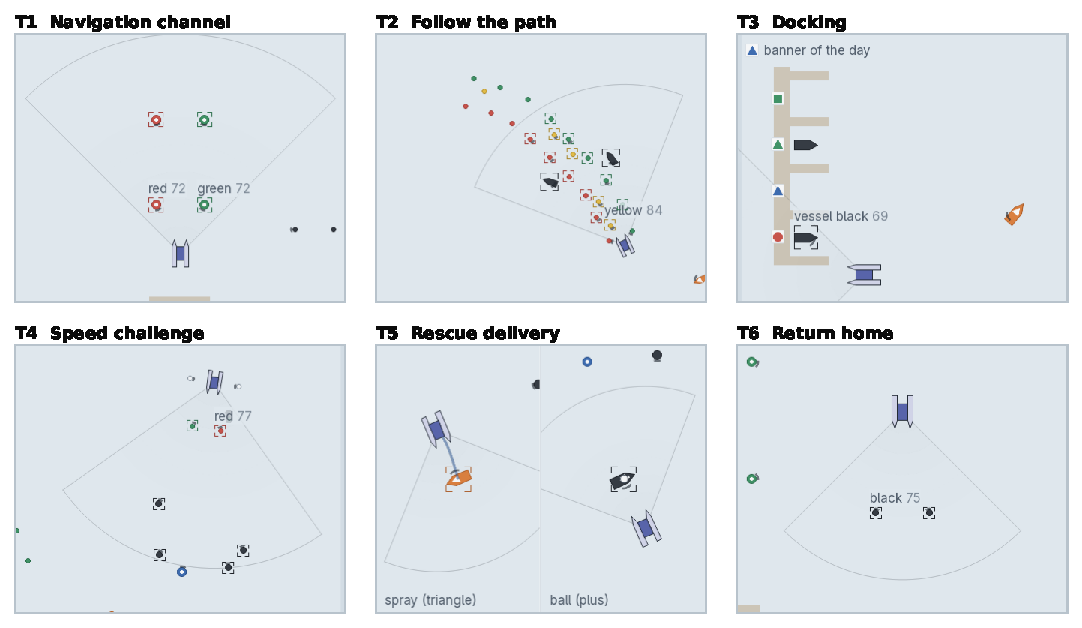
\includegraphics[width=\linewidth]{fig_tasks.pdf}
\caption{The six tasks as simulated. The grey wedge is a boat's camera field of view ($90^\circ$, 18\,m); brackets mark camera detections with class and confidence (\%); short dark arcs are lidar returns ($360^\circ$, 20\,m). Objects at the panel edges belong to neighbouring tasks.}
\label{fig:tasks}
\end{figure}

The camera's detection probability falls with range and off-axis angle, and it confuses classes (red with orange, triangle with plus) more at long range; banners are readable only within 7\,m and from the front. A per-boat tracker fuses camera and lidar detections into objects with class probabilities and de-duplicated counts. Boats broadcast a compact digest of their maps once per second, so each boat's \emph{team map} merges what it has seen with what it has heard.

With a \emph{perfect} radio every message arrives, after the 0.5--3\,s latency; the \emph{unreliable} radio adds the burst losses described above. Every 2\,s, each boat's strategy chooses among the tasks its map supports. The strategies differ only in how they choose:
\begin{itemize}
\item The \emph{greedy} strategy (P0) takes the nearest task. The \emph{selfish race} (P1) values a task only if no teammate claiming it is predicted to arrive first. (A \emph{claim} is the task a boat announces it is heading to, broadcast with its estimated time of arrival, ETA.)
\item \emph{Team-aware} boats maximize the difference reward \eqref{eq:dr} minus travel cost,
\begin{equation}
U_i(j)=V_j\,s_i(1-s_{-i})-\lambda\,\mathrm{ETA}_i(j),\qquad s_i=F_{\mathcal N}\!\Big(\tfrac{T_{\rm run}-t-\mathrm{ETA}_i}{4\,\mathrm s+0.12\,\mathrm{ETA}_i}\Big),\label{eq:mc}
\end{equation}
with $\lambda=2$ points per second and $s_{-i}=1-\prod_k(1-s_k)$ over teammates $k$ believed to be heading to $j$. Here $s_i$ is the chance of finishing before the end of the run, modelling the arrival time as normal around the ETA with a spread that grows with distance; $F_{\mathcal N}$ is the standard normal distribution function. A $2\times2$ design varies the travel-time model (graph or control-aware) and the beliefs about teammates: P2 (graph, naive), A1 (graph, age-aware), A2 (control-aware, naive), P3 (control-aware, age-aware). A \emph{naive} boat trusts a teammate's last claim as received; an \emph{age-aware} boat multiplies $s_k$ by $e^{-\max(0,\theta-1.5)/6}$ for a claim $\theta$ seconds old.
\item \emph{Reservations} (R3), new in this study, treats a claim as a reservation, trusted in full until the claimant's own announced completion time plus a margin ($\max(5\,\mathrm s,\,0.25\times$ the claimant's planned ETA$)$), and only then decayed. It is otherwise identical to A2 and P3.
\item \emph{Central assignment} (P4) solves the joint assignment every 2\,s with the Hungarian algorithm~\cite{kuhn1955}, which matches each boat to at most one task so that the total utility is largest, in $O(n^3)$. It sees exact positions and its commands arrive instantly, information no real boat has, so it serves as an \emph{oracle} benchmark. The \emph{leader on radio} (P5), new here, runs the same solver on one boat, using only that boat's own map and teammates' last \emph{received} positions; each assignment reaches a teammate only when that teammate hears a newer leader message.
\end{itemize}

\begin{figure}[t]
\centering
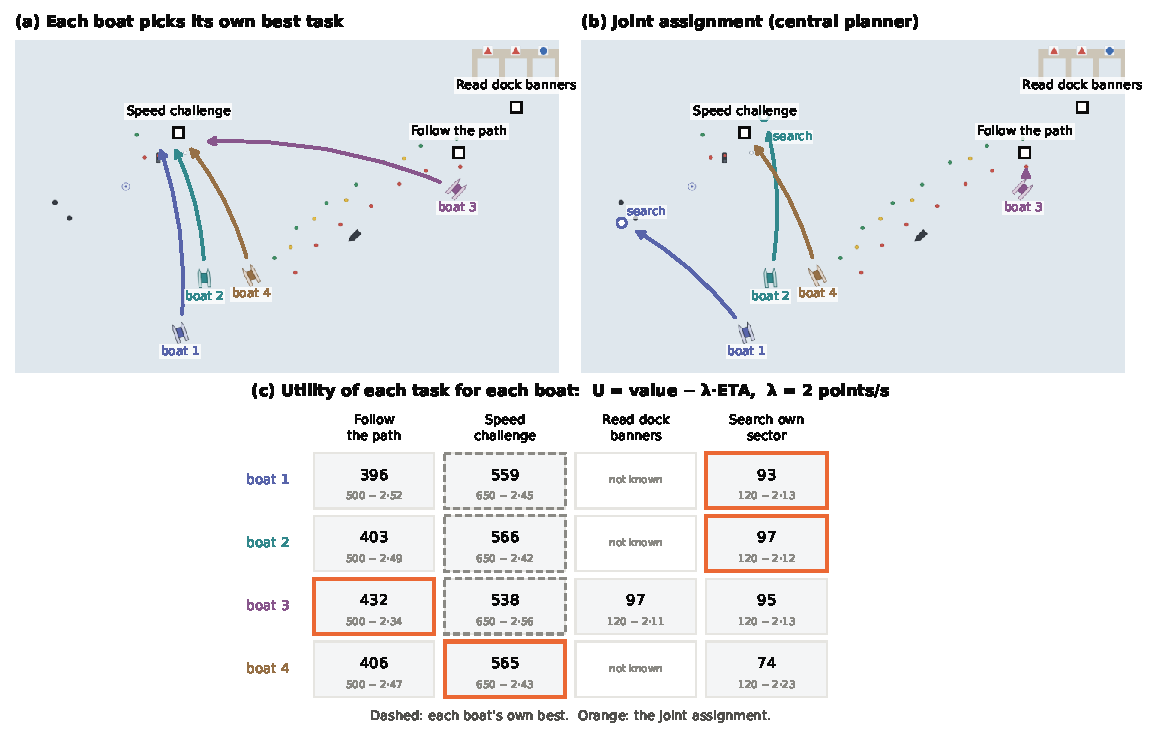
\includegraphics[width=\linewidth]{fig15_decision.pdf}
\caption{One decision on a generated course (course 11, $t=36$\,s; utilities computed by the simulator). \textbf{(a)} Each boat takes its own best task, and all four race for the speed challenge. \textbf{(b)} The joint assignment splits them. \textbf{(c)} The utility matrix behind both: value $-\ 2\times$ETA in seconds. ``Not known'' means the task is not yet on that boat's map. ``Search own sector'' is a personal option, so it never conflicts.}
\label{fig:decision}
\end{figure}

Figure~\ref{fig:decision} freezes a real decision. Every success probability is 1 here, so each utility is value minus $\lambda\cdot$ETA. Choosing alone, all four boats pick the speed challenge, their largest entry; it scores once, so the team nets one speed challenge (565) minus three wasted trips, about 277. The joint assignment picks one entry per row, each column at most once, to maximize the sum ($93+97+432+565\approx1{,}187$). It gives the speed challenge to boat 4 (565) rather than boat 2 (566): once boat 3 takes the path, boat 2's best remaining option (searching, 97) is worth more than boat 4's (74), so the total is larger this way. Joint assignment prices \emph{opportunity cost}, which no single row can see. A team-aware boat reaches a similar split through \eqref{eq:dr}, provided it hears its teammates' claims in time.

\subsection*{The coordination layer}\label{sec:layer}
Porting the strategies to this course exposed failures that no strategy could fix, because they lived in shared machinery. We repaired them in a layer that all strategies use; \S\ref{sec:q3} measures each piece on fresh courses.
\begin{itemize}
\item With \emph{sensed deconfliction}, when two boats claim the same single-boat task, the farther one yields once it \emph{sees} the other within 15\,m, and avoids that task for 40\,s.
\item In \emph{recon sectors} (for reconnaissance), the basin is split into one stripe per boat, and unexplored water in a boat's own stripe is worth more; boats head for the nearest edge of unexplored water, in the spirit of frontier exploration~\cite{yamauchi1997,burgard2005}.
\item With \emph{bonus-aware values}, because the return bonus requires every task type to be attempted, a type nobody has tried gets a 300-point premium.
\item With \emph{queue-aware return}, a boat heads home when $t+\mathrm{ETA}^{\rm home}+25+7k>T_{\rm run}$, where $T_{\rm run}$ is the run length, 25\,s is a safety margin, and each of the $k$ teammates expected at the 3.2\,m home gate before it adds about 7\,s, the time one boat takes to pass the gate.
\item In \emph{bay inference}, a vessel seen in a bay rules it out; when all bays but one are ruled out, the last is inferred to match.
\end{itemize}
Smaller repairs are documented in the code.\footnote{Each boat gets its own copy of T1, which every boat must pass before scoring; the central solver is masked so that it cannot give one boat's own channel pass or trip home to another; a boat holding for the T4 start light faces the light; and right-of-way rules prevent deadlocks at narrow gates. On the courses used to find these defects, the layer raised the central planner's mean score from 2{,}549 to 5{,}976 points.}

% =====================================================================================
\section{How the experiments are compared}
\label{sec:stats}
Every experiment is \emph{paired}. A course seed fixes the map, currents, task positions, sensor noise and every dropped radio packet, and every strategy plays every course with these identical random inputs (common random numbers~\cite{yang1991}). For strategies $A$ and $B$ we analyse the per-course differences $d_w=A(w)-B(w)$. Pairing matters because
\[
\operatorname{Var}(\bar d)=\frac{\sigma_A^2+\sigma_B^2-2\rho\,\sigma_A\sigma_B}{N},
\]
where $N$ is the number of courses, $\sigma_A,\sigma_B$ the spreads of each strategy's score across courses and $\rho$ their correlation. Hard courses are hard for every strategy, so $\rho$ is large. In the preregistered study (\S\ref{sec:q2}) pairing cut the spread of differences from 28.5 to 19.3 points for one contrast and from 26.9 to 10.9 for the other, variance ratios of 2.2 and 6.1, so it was as good as running two to six times as many courses.

We test whether a mean difference is zero with a sign-flip randomization test. If two strategies are interchangeable, each $d_w$ is as likely to be negative as positive, so we flip signs at random 100{,}000 times and ask how often the flipped mean is as extreme as the observed one. The test needs only that symmetry, not normality; the differences here are moderately skewed (skewness 0.2--0.9), and paired $t$-tests agree with every result reported. Intervals, written $[\,\cdot,\cdot\,]$ after an estimate, are 95\% bootstrap confidence intervals (CI): the range the mean would span if we resampled the courses. They are \emph{not} adjusted for testing several contrasts at once. The $p$-values are, with Holm's procedure~\cite{holm1979}, a step-down correction that keeps the chance of any false positive within a named \emph{family} of tests at 5\%. We report the effect size $d_z=\bar d/s_d$, with $s_d$ the standard deviation of the differences, the mean difference in units of its own spread; if differences are roughly normal, a strategy with effect $d_z$ wins a random course with probability about $F_{\mathcal N}(d_z)$.

Table~\ref{tab:studies} lists the studies. The first predates the RoboBoat course: a \emph{preregistered} experiment on an earlier, abstract course, whose hypotheses and analysis were fixed in writing, with a cryptographic hash recorded, before any held-out data were simulated (\S\ref{sec:q2}). An \emph{ablation} switches off one component at a time to measure what it contributes; the \emph{return rush} is the Braess experiment of \S\ref{sec:q1}.

\begin{table}[t]
\centering\small
\caption{The studies, in the order they were run. H1 and H2 are the two preregistered hypotheses (\S\ref{sec:q2}); welfare is points minus energy and contact penalties. ``Plan fixed'' means the hypotheses, outcomes and test family were written down before the held-out data were simulated. All studies use courses never used during development.}
\label{tab:studies}
\begin{tabular}{p{0.34\linewidth}lp{0.36\linewidth}}
\toprule
Study & Plan fixed & Family and outcome\\\midrule
Abstract course, 400 worlds & preregistered (hashed) & H1, H2; welfare; Holm over 2\\
RoboBoat course, 200 courses, 4 and 2 boats & yes & 6 contrasts per outcome; Holm\\
New strategies P5, R3 (same 200 courses) & yes & 4 contrasts per fleet size; Holm\\
Coordination-layer ablation, 100 courses & script fixed & 5 components per strategy; Holm\\
Robustness (harsher radio, slower boats) & yes & descriptive, unadjusted\\
Return rush and coupling sweep & selection rule fixed & exploratory; key points re-validated on fresh seeds\\
\bottomrule
\end{tabular}
\end{table}

Points on the RoboBoat course need one more remark. The return bonus is worth about twice a run's task points and is all-or-nothing, so for one strategy on one course it behaves like a coin flip with standard deviation of about 2{,}400 points. That noise swamps differences of a hundred task points, so we compare strategies on \emph{task points} (the score without the bonus) and report total points and bonus rates alongside.

% =====================================================================================
\section{When does the game describe the fleet?}
\label{sec:q1}
We built the harbour into the end of the course, as a \emph{return rush}. After the tasks, four boats race home from $S$, the exit of the task area, to $T$, the home gate. Junction $A$ is where the west channel ends and open water begins; junction $B$ is where open water ends and the east channel begins. Each boat goes either through a single-file buoy channel (\mbox{$S\!\to\!A$}) and open water (\mbox{$A\!\to\!T$}), or through open water (\mbox{$S\!\to\!B$}) and a second channel (\mbox{$B\!\to\!T$}). A gap in a spill boom, the shortcut, joins $A$ to $B$. \emph{Fleet time} is the sum of the four boats' times from $S$ to $T$; the single-file channels and open-water legs replace the canals and open legs of the harbour. We measured each edge's travel time with $k=1,\dots,4$ boats from scripted runs, solved the resulting congestion game exactly, and chose in advance the geometry that predicted the largest paradox. The game predicted that opening the shortcut would send all four boats down it and raise fleet time from 349.4\,s to 363.6\,s, and that tolls would bring it to the optimum of 338.5\,s, which uses the shortcut for two boats (so the PoA is $363.6/338.5=1.074$).

\begin{figure}[t]
\centering
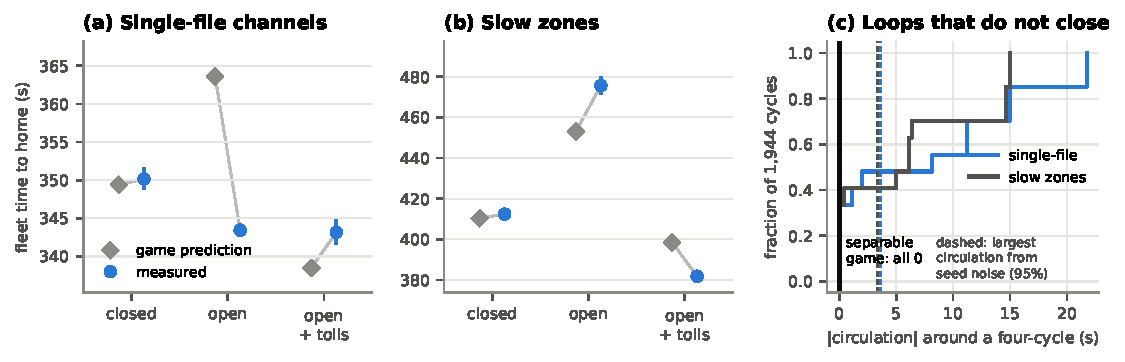
\includegraphics[width=\linewidth]{fig_physical.pdf}
\caption{\textbf{(a, b)} The calibrated congestion game's prediction (diamonds) against the simulated fleet (dots: mean and 95\% interval over 100 paired seeds; some intervals are narrower than the marker), for single-file channels and for slow zones. With queues the predicted paradox reverses; with slow zones it appears, larger than predicted. \textbf{(c)} Circulation around all 1{,}944 four-cycles of the \emph{measured} route games. The calibrated separable game has circulation exactly zero; the measured games exceed seed noise (dashed) on more than half the cycles. About a third of cycles are zero by symmetry (swapping boats on the same route).}
\label{fig:physical}
\end{figure}

The prediction failed. On 100 paired seeds, opening the shortcut \emph{lowered} fleet time by 6.7\,s [5.6, 8.0], and tolls added nothing measurable (Fig.~\ref{fig:physical}a). The last boat home did arrive 7.9\,s later with the shortcut open, which matters for a bonus that needs every boat home. The model's assumptions are what failed. When single-file queues are replaced by \emph{slow zones}, open water in which every boat's speed limit is $v_0/(1+\beta(k-1))$, with $v_0$ the free speed, $\beta$ a congestion coefficient and $k$ the number of boats inside, so that a crowd slows down together the way road traffic does, the paradox appears. Opening the shortcut raised fleet time by 63.2\,s [59.2, 67.3] against a predicted 42.7\,s, and tolls cut it by 93.8\,s (Fig.~\ref{fig:physical}b). That geometry, too, was chosen by a rule fixed before measuring. (A further geometry, chosen after screening, showed a paradox of $+7.3$\,s on fresh seeds against a predicted $+0.2$\,s; we do not count it as confirmation.)

The reason is that travel times depend on traffic elsewhere. A single-file channel admits one boat every $h$ seconds, its service interval. Boats on the shortcut route have just come through the west channel, so they reach the east channel already spaced about $h$ apart, while boats arriving through open water arrive bunched. We injected four boats into the east channel at controlled spacing $\Delta$ and found mean delays that fall linearly and vanish at $\Delta\approx h$, as a deterministic queue predicts (Fig.~\ref{fig:coupling}a). If four boats arrive $\Delta$ apart and are served one every $h$ seconds, the $k$-th waits $(k-1)(h-\Delta)$, so the average wait is $1.5\max(0,h-\Delta)$. The measured curves follow this law but are shifted about 2\,s lower, because boats that start ``together'' actually arrive about 1.8\,s apart. The service interval itself comes from the dynamics: $h\approx5.4\,\mathrm s+L/(1.65\,\mathrm{m/s})$ for a channel of length $L$, where the constant is the time to accelerate out of the hold and clear the exit. So the east channel's cost depends on how boats \emph{arrive}, which depends on which route they took. Measured at $k=4$, the east channel costs 29.8\,s for boats arriving through the shortcut against 35.6\,s for bunched arrivals. We define a coupling index $\kappa=1-\dfrac{D_{\rm spaced}}{D_{\rm bunched}}$, where $D$ is the east channel's extra delay at $k=4$ (its time minus the one-boat time) for boats arriving spaced from the shortcut or bunched from open water. So $\kappa=0$ when the channel's congestion is independent of where its boats came from, and $\kappa=1$ when upstream spacing removes it entirely. The queue course has $\kappa=0.67$; the slow-zone course, 0.20.

\begin{figure}[t]
\centering
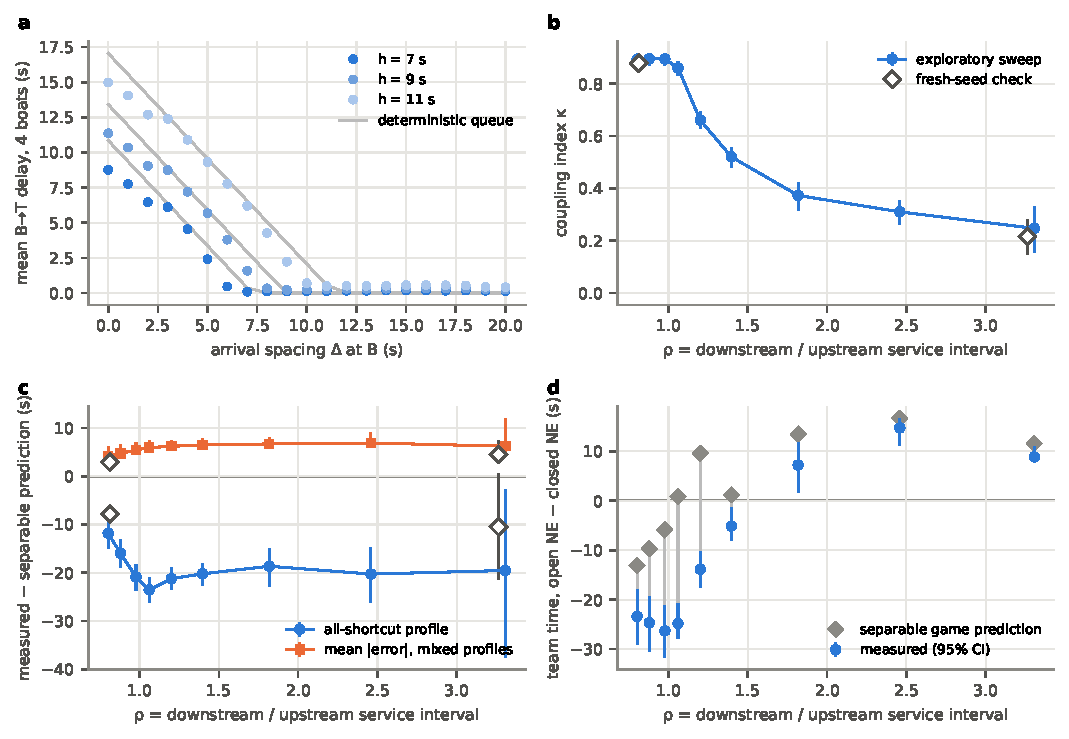
\includegraphics[width=\linewidth]{fig18_coupling.pdf}
\caption{Cross-route coupling in the return rush. \textbf{(a)} Mean delay of four boats in a single-file channel against their arrival spacing $\Delta$, for three service intervals $h$; grey lines are the deterministic queue law. \textbf{(b)} Coupling index $\kappa$ against $\rho$, the ratio of downstream to upstream service intervals (exploratory sweep, filled dots; open diamonds re-measured on fresh seeds). \textbf{(c)} Measured minus predicted fleet time for the all-shortcut profile (blue, signed) and the mean absolute error over mixed profiles (orange). \textbf{(d)} Predicted (grey diamonds) and measured (blue) Braess effect, shortcut-open minus shortcut-closed fleet time, across the sweep.}
\label{fig:coupling}
\end{figure}

To see when the separable model works, we slowed the downstream channel with a speed limit, varying $\rho$, the ratio of downstream to upstream service intervals, from 0.8 to 3.3 (an exploratory sweep, with the end points re-measured on fresh seeds). Coupling falls steadily, from $\kappa=0.89$ to 0.25 (Fig.~\ref{fig:coupling}b). The model's absolute error does not shrink with it: the measured fleet time for the all-shortcut profile is roughly 20\,s \emph{lower} than predicted across the sweep (Fig.~\ref{fig:coupling}c). A fresh-seed re-measurement at $\rho=3.3$ gives $-10$\,s [$-21$, 1]. The error does not shrink because the head start that upstream spacing gives is bounded by the upstream service interval, so it stays roughly fixed in seconds. What changes is the size of the effect the model is trying to predict. For $\rho\lesssim1.4$ the predicted paradox is smaller than the error and the measured sign is often reversed; from $\rho\approx1.8$ the predicted paradox outgrows the error and the signs agree (Fig.~\ref{fig:coupling}d). The separable game predicts Braess's paradox correctly only when the downstream bottleneck is roughly twice as slow as the upstream one.

With these costs, the circulation test of \S\ref{sec:curl} becomes a measurement. There are 15 ways to split four boats among three routes (the \emph{route-count profiles}); for each we measured the mean cost of each route, built the symmetric four-boat game, and computed the circulation around all 1{,}944 four-cycles (Fig.~\ref{fig:physical}c). The calibrated separable game gives exactly zero on every cycle, as Theorem~\ref{thm:rosenthal} guarantees. In the measured queue game the largest circulation is 21.7\,s [20.3, 23.2], six times the largest value produced by \emph{seed noise} alone (3.6\,s, the 95th percentile of the maximum when the route costs are re-estimated from resampled seeds), and 52\% of its cycles exceed three standard errors. (About a third of all cycles are zero by symmetry, because swapping two boats on the same route changes nothing.) One explicit cycle: from (west, west, west, east), boat 1 switches west$\to$east ($-1.78$\,s for it), boat 2 switches west$\to$shortcut ($-10.77$\,s), boat 1 switches back ($-7.41$\,s) and boat 2 switches back ($-1.78$\,s). The loop returns to its start, yet the movers' cost changes, all four of them improvements on average, sum to $-21.7\pm0.7$\,s. By the four-cycle theorem, no exact potential exists.

There is a stronger statement. In route counts (west, east, shortcut), the measured queue game contains the cycle
\[
(1,2,1)\xrightarrow{\ \text{east}\to\text{west}\ }(2,1,1)\xrightarrow{\ \text{shortcut}\to\text{east}\ }(2,2,0)\xrightarrow{\ \text{west}\to\text{shortcut}\ }(1,2,1),
\]
in which every move strictly improves the mover's time, by 7.4, 3.6 and 10.8\,s, each interval excluding zero. Each step moves one boat, so with labelled boats it becomes a closed improvement path of six moves before every boat is back on its original route. A finite game with any potential that preserves the \emph{sign} of improvements (an ordinal or generalized-ordinal potential) cannot contain a strict improvement cycle, since the potential would decrease all the way around a loop. So the measured game, with each route's mean cost in each profile, has no such potential. Checking all 15 profiles directly, none is a \emph{pure} Nash equilibrium (one in which each boat simply picks a route, rather than randomizing), so selfish boats responding to these costs never settle. The slow-zone game is not separable either: its circulations reach 15.0\,s, and 59\% of its cycles exceed three standard errors. Its coupling is weaker ($\kappa=0.20$), and the improvement cycles found there include a step within seed noise, so there we claim only the failure of an exact potential. What distinguishes it from the queue course is that its predicted paradox is large enough to survive the model error.

% =====================================================================================
\section{Does a better model of physics or information help?}
\label{sec:q2}
\subsection{A better clock rarely changes the decision}
The first study, preregistered, used an earlier, abstract course with islands, one-lane channels, and generic tasks with deadlines in place of the RoboBoat tasks. It tested two hypotheses on 400 held-out worlds. H1: control-aware travel times beat graph travel times (P3 against A1, perfect radio). H2: age-aware beliefs beat naive ones (P3 against A2, unreliable radio). The outcome was welfare, points minus energy and contacts.

\begin{table}[h]
\centering\small
\caption{Preregistered contrasts on the abstract course ($N=400$ held-out worlds; interval unadjusted, $p$ Holm-adjusted over the two). $\Delta W$ is the mean per-world difference in welfare; ``wins'' is the share of worlds in which P3 scored higher.}
\label{tab:primary}
\begin{tabular}{llrrrr}
\toprule
 & Contrast & Mean $\Delta W$ [95\% CI] & $d_z$ [95\% CI] & $p_{\rm Holm}$ & wins\\\midrule
H1 & P3 $-$ A1, perfect radio & $-1.00$ [$-2.84$, $0.93$] & $-0.05$ [$-0.15$, $0.05$] & 0.60 & 44\%\\
H2 & P3 $-$ A2, unreliable radio & $-0.01$ [$-1.07$, $1.05$] & $-0.00$ [$-0.10$, $0.10$] & 0.98 & 43\%\\\bottomrule
\end{tabular}
\end{table}

Both failed, and both intervals exclude the effect size the study was designed to detect, $d_z=\pm0.25$ (Table~\ref{tab:primary}). The control-aware model does predict travel time better, with mean absolute error 7.5\,s against 8.4\,s, and it is better for routes of every degree of twistiness (total turning angle). But a boat acts only on the option that ranks first. Let $\delta_j$ be the difference between the two models' travel-time estimates for task $j$. If the utilities differ only through travel time, the chosen task $j^*$ changes to some $j'$ only when
\[
\lambda\,\big|\delta_{j^*}-\delta_{j'}\big| \;>\; U_i(j^*)-U_i(j'),
\]
that is, when the clocks' disagreement about two options exceeds the margin between them. Replaying 29{,}032 decisions with the graph model in place of the control-aware one, the same task was chosen 93.6\% of the time, and 89\% even when the top two options were within one point. When the choices did differ, the later decisions that changed as a result could swing a world by $\pm50$ points, but such swings helped as often as they hurt. On the RoboBoat course the same contrast gives $+66$ task points [12, 122]; the unadjusted interval excludes zero, but after Holm's correction for the six planned tests $p=0.058$.

\subsection{How stale information causes duplicated effort}
On the abstract course, discounting stale messages made no difference. On the RoboBoat course it does harm. With four boats and an unreliable radio, P3 scores 111 task points fewer [58, 163] than A2, which is identical except that it never discounts (Holm $p<0.001$; Table~\ref{tab:v2}). The reason is the difference reward \eqref{eq:dr}. Discounting a teammate's claim lowers $s_{-i}$, which \emph{raises} the task's value to a second boat: the boat charges itself too small a toll and goes. P3 boats had to abandon a duplicated claim 7.1 times per run on the 200 courses, against 2.0 for A2; the central oracle, which never assigns a task twice, had none.

The natural repair is to discount only claims that are genuinely stale. Our reservation strategy R3 trusts a claim fully until the claimant's announced completion time plus a margin. It did not help: R3 is level with P3 ($+27$ task points [$-30$, 81]) and still 84 below A2 (Holm $p=0.002$), abandoning 4.1 duplicated claims per run. The reason is that the announced time is when a boat expects to \emph{reach} its task, not when it will finish. 97\% of speed-challenge claims finish more than 5\,s after the announced time, while the boat holds for the green light, so any rule that reads lateness as abandonment withdraws trust from boats that are still working.

What does signal abandonment is \emph{silence}, since every status message re-asserts the sender's claim. A heartbeat lease (L3, designed after the diagnostic above and labelled exploratory) keeps a claim valid while the claimant keeps broadcasting it, and lets it decay only after 8\,s of silence, longer than a typical loss burst. It recovers part of the loss: 71 task points over P3 [20, 121] (Holm $p=0.013$), with 3.0 duplicates per run. It still trails A2, which never discounts a claim, by 40 [1, 81]; with a perfect radio no claim goes silent for 8\,s and L3 coincides with A2. The four rules line up by how readily they doubt a teammate:
\begin{center}\small
\begin{tabular}{lccc}
\toprule
Rule & doubts a claim & duplicates per run & task points\\\midrule
P3 & by message age & 7.1 & 2{,}307\\
R3 & by lateness & 4.1 & 2{,}334\\
L3 & after 8\,s of silence & 3.0 & 2{,}377\\
A2 & never & 2.0 & 2{,}418\\\bottomrule
\end{tabular}
\end{center}
(R3 and P3 are not significantly different.) In this fleet a claim is incomplete information but rarely wrong information: boats give up tasks only by finishing them or by yielding, and both are announced. Trusting a claim until it is released was the better rule here, and \eqref{eq:dr} then charges the correct toll.

\begin{table}[t]
\centering\small
\caption{Four boats on 200 RoboBoat courses: planned paired contrasts on task points (unadjusted 95\% intervals; $p$ Holm-adjusted within each family). The plan for Family~1 named total points as the primary outcome; we show task points for the reason given in \S\ref{sec:stats}. On total points, P4 and P1 beat P3 under the unreliable radio ($+826$ and $+786$; Holm $p\le0.006$) and the other Family~1 contrasts are not significant.}
\label{tab:v2}
\begin{tabular}{llrrr}
\toprule
Contrast & Radio & Task points [95\% CI] & $p_{\rm Holm}$ & $d_z$\\\midrule
\multicolumn{5}{@{}l}{\emph{Family 1: planned contrasts (Holm over 6)}}\\
P3 $-$ A1 (dynamics ETA) & perfect & $+66$ [$+12$, $+122$] & 0.058 & $+0.17$\\
P3 $-$ A2 (age-aware beliefs) & unreliable & $-111$ [$-163$, $-58$] & $<0.001$ & $-0.29$\\
P4 $-$ P3 (central oracle) & perfect & $+23$ [$-29$, $+81$] & 0.825 & $+0.06$\\
P4 $-$ P3 (central oracle) & unreliable & $+161$ [$+102$, $+226$] & $<0.001$ & $+0.36$\\
P1 $-$ P3 (selfish race) & perfect & $+20$ [$-31$, $+69$] & 0.825 & $+0.06$\\
P1 $-$ P3 (selfish race) & unreliable & $+120$ [$+65$, $+174$] & $<0.001$ & $+0.31$\\
\midrule\multicolumn{5}{@{}l}{\emph{Family 2: new strategies, planned (Holm over 4)}}\\
R3 $-$ P3 (reservations) & unreliable & $+27$ [$-30$, $+81$] & 0.346 & $+0.07$\\
R3 $-$ A2 & unreliable & $-84$ [$-132$, $-36$] & 0.002 & $-0.24$\\
P4 $-$ P5 (privileged information) & unreliable & $+244$ [$+178$, $+312$] & $<0.001$ & $+0.50$\\
P5 $-$ P3 (leader on radio) & unreliable & $-83$ [$-153$, $-14$] & 0.042 & $-0.16$\\
\midrule\multicolumn{5}{@{}l}{\emph{Family 3: heartbeat lease, exploratory (Holm over 2)}}\\
L3 $-$ P3 (heartbeat lease) & unreliable & $+71$ [$+20$, $+121$] & 0.013 & $+0.20$\\
L3 $-$ A2 & unreliable & $-40$ [$-81$, $-1$] & 0.047 & $-0.14$\\
\bottomrule
\end{tabular}
\end{table}

% =====================================================================================
\section{When does coordination structure matter?}
\label{sec:q3}
\begin{figure}[t]
\centering
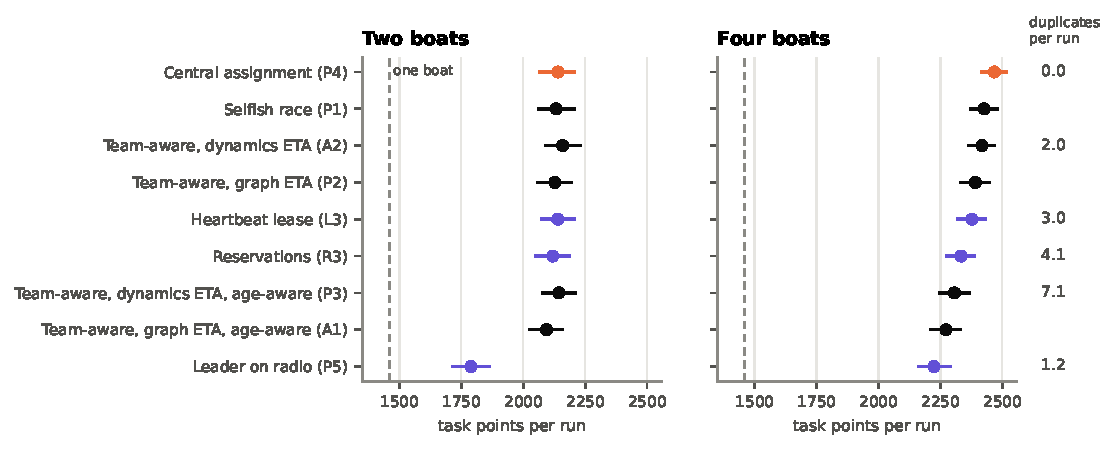
\includegraphics[width=\linewidth]{fig_league.pdf}
\caption{Task points per run with an unreliable radio, on the same 200 courses for every fleet size (mean and 95\% interval). Orange: central oracle; violet: strategies new in this study; black: the others. Right: duplicated claims abandoned per run with four boats. Greedy is off-scale (869 task points with two boats, 1{,}280 with four). The dashed line marks a single boat (1{,}460 task points).}
\label{fig:league}
\end{figure}

Whether coordination matters depends on fleet size. Figure~\ref{fig:league} compares the strategies on the same 200 courses with two and four boats. With the A2 strategy, a single boat earns about 1{,}460 task points, a second boat adds about 700, and two more add only about 260. The decentralized strategies and the oracle separate only in the larger fleet. With two boats, none of them differs significantly from another, and every planned contrast among them lies within about $\pm110$ task points of zero; only greedy and the leader-on-radio planner fall behind. With four boats, the central oracle beats P3 by 161 task points [102, 226] (Holm $p<0.001$), and the strategies that rarely duplicate (P4, A2, P1) lead.

Lemma~\ref{lem:ext} explains the difference. The gap between what a boat sees and what the fleet pays is the externality it imposes on boats \emph{already there}. With two boats on a large course, in separate search sectors, there are rarely any boats already there: P3 boats abandoned a duplicated claim 1.6 times per run with two boats (in a 30-course check), against 7.1 with four. With so few conflicts, every sensible rule makes nearly the same choices, and the limit is how much water two boats can cover in the time available. Coverage is also why two-boat fleets earned the return bonus in only 30--40\% of runs: two boats often cannot attempt every task type and get home within 300\,s.

The central oracle P4 differs from the decentralized boats in two ways at once: it solves the joint assignment, and it has exact positions and instant commands. The leader-on-radio planner P5 runs the same solver with only what one boat knows and hears. With four boats it trails the oracle by 244 task points [178, 312] and even trails P3 by 83 (both Holm $p<0.05$); with two boats the gap to the oracle is 351 task points [273, 431]. P5 stays far behind even with a perfect radio, so the cause is not lost packets alone. The leader knows only what reaches it as compressed map digests, and its teammates act only on its orders. A post-hoc leader variant on the abstract course found the same: it recovered none of the oracle's lead under a perfect radio. Most of what a central planner gains comes from privileged information and instant commands, not from solving the assignment.

Switching off each component of the coordination layer (\S\ref{sec:layer}) on 100 further courses (Fig.~\ref{fig:ablation} for four boats) shows that decentralized boats depend on one of them. Without sensed deconfliction, P3 loses 1{,}245 total points with four boats and 1{,}294 with two (264 and 333 task points; all Holm $p<0.001$), and its bonus rate roughly halves. Duplicates are rare with two boats, but each one wastes half the fleet for a minute. Central assignment never assigns one task twice, so deconfliction does nothing for it. P4's gains come from rules that protect the return bonus: bay inference (+696 total points) and queue-aware return (+571) with four boats, both of which change task points by under 50; neither matters with two. Recon sectors and bonus-aware values had no significant effect for either strategy.

\begin{figure}[t]
\centering
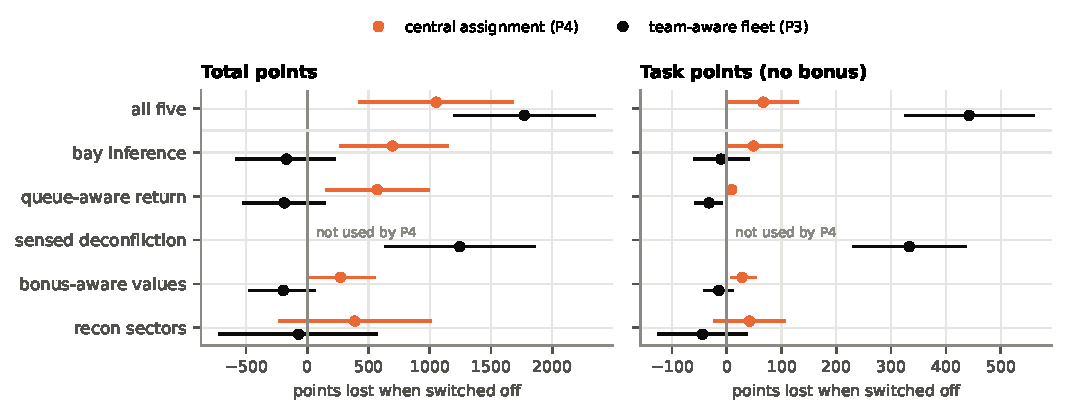
\includegraphics[width=\linewidth]{fig13_v2_ablation.pdf}
\caption{Points lost when each coordination component is switched off (four boats, unreliable radio, paired over 100 fresh courses; mean and 95\% interval). Orange: central oracle P4; black: P3. Positive values mean the component helps.}
\label{fig:ablation}
\end{figure}

The main contrasts held under two harsher settings. On 100 new courses, once with a radio that drops into its bad state twice as often and delivers messages up to 5\,s late, and once with boats a quarter slower, the central oracle still led P3 by 147 and 218 task points, and A2 still led it by 133 and 157 (unadjusted intervals excluding zero). The lease again fell between them, and P3 again made the most duplicated trips.


% =====================================================================================
\section{Discussion: when is a game a good description of robots?}
\label{sec:disc}
The theory of \S\ref{sec:math} describes a fleet in which costs are known numbers, each edge's cost depends only on its own load, and boats move one at a time on correct information. None of these holds exactly for real boats, but the experiments show that they matter very differently, and the differences say something about when a game is the right model.

The first assumption barely matters. Turning limits and currents make a route's true travel time depend on its shape, and a dynamics-aware estimate is measurably better than path length divided by speed. Yet a boat acts only on the option that ranks first, and an estimate that is better on average rarely changes that ranking. Both the preregistered study and the RoboBoat replication found that refining the costs hardly moved the fleet. An imperfect cost model is tolerable as long as it orders the options correctly.

The second assumption is where the model breaks, and it breaks in a way the mathematics can detect. Single-file queues make a channel's delay depend on how boats arrive, and so on the routes they took to get there. A congestion game has no room for that dependence, and the measured costs show it: the separable prediction is off by tens of seconds, the paradox reverses wherever its predicted size is smaller than that error, and the four-cycle circulations, which must vanish in any potential game, sit far above noise. The queue course even contains a strict improvement cycle and has no pure equilibrium, so selfish boats responding to its true costs would never settle. Congestion that slows a group together couples the edges less. That game is still not a potential game, but its coupling is weak enough that the paradox shows through, at one and a half times its predicted size. The circulation test turns ``is this a potential game?'' from an assumption into a measurement that any team logging per-profile costs can repeat.

The third assumption fails through the toll. The difference reward charges a boat for value its teammates would produce anyway, and that charge depends on $s_{-i}$, a belief about what teammates are doing. Every rule that discounted a teammate's claim, whether for the message's age, for the teammate's lateness or after a long silence, undercharged for tasks that were in fact taken, and duplicated trips rose in step with how readily the rule doubted. In this fleet claims were incomplete but rarely wrong, so the simplest policy was best: trust a claim until it is released. The same externality explains why fleet size matters. With two boats there is rarely another boat on the same task, and every sensible strategy ties; with four, duplicated trips become common, and strategies that avoid them win. A central planner's lead, in turn, comes mostly from what it knows and how fast its commands arrive, not from solving the assignment.

For a team writing the software for a two-boat entry, the choice of coordination rule matters little, as long as the pair never works the same task twice. Broadcast claims and treat them as binding until released; resolve the rare duplicate at once, by sight if necessary; and spend engineering effort on task execution, search and return timing rather than elaborate allocation. With a reliable link, one planner assigning both boats avoids duplicates entirely. On a shared route home, a single-file gate meters traffic and works against Braess's paradox unless the bottleneck after it is much slower; a slow, crowded zone does not meter anything.

Several limits apply. The boat and sensor models are simplified and unvalidated against hardware. The course implements the 2025 task set, not the 2026 one, and the multi-boat scoring rules are our interpretation. The return-rush experiments use one course layout and four boats, and the coupling sweep is exploratory with its end points re-validated. The new strategies P5 and R3 were planned; the lease L3 was designed after seeing R3's result.

Everything needed to reproduce the study is in the project repository: the code, simulator, every episode table, the preregistration and each analysis plan (written before the corresponding results), and the scripts that regenerate every number and figure. The interactive simulator (\texttt{rb2.viz.app2}) shows a fleet working the course; a replay (\texttt{rb2.viz.braess\_demo}) shows the return rush with the shortcut closed and open.


\bibliographystyle{plainnat}
{\footnotesize\setlength{\bibsep}{1pt}
\bibliography{references}}
\end{document}
